\subsubsection{Blockdiagramm}
Das Blockdiagramm beschreibt den Zusammenhang der einzelnen Komponenten. In Abbildung \ref{fig:blockdiagramm} wird dies dargestellt. Die externe Steuerungseinheit (Notebook) greift über WLAN auf das Raspberry Pi zu. Dieses kommuniziert mit der PI-Kamera für die Detektion des Korbes. Zudem greift das Pi auch auf das Freedom Board zu, welches wiederum zuständig für alle Motoren ist. Die Turmausrichtung übernimmt der Stepper, die Beschleunigung des Schwungrades ist Sache des BLDC-Motors und für den Ballnachschub ist der DC-Motor zuständig.

\begin{figure}[h!]
\centering
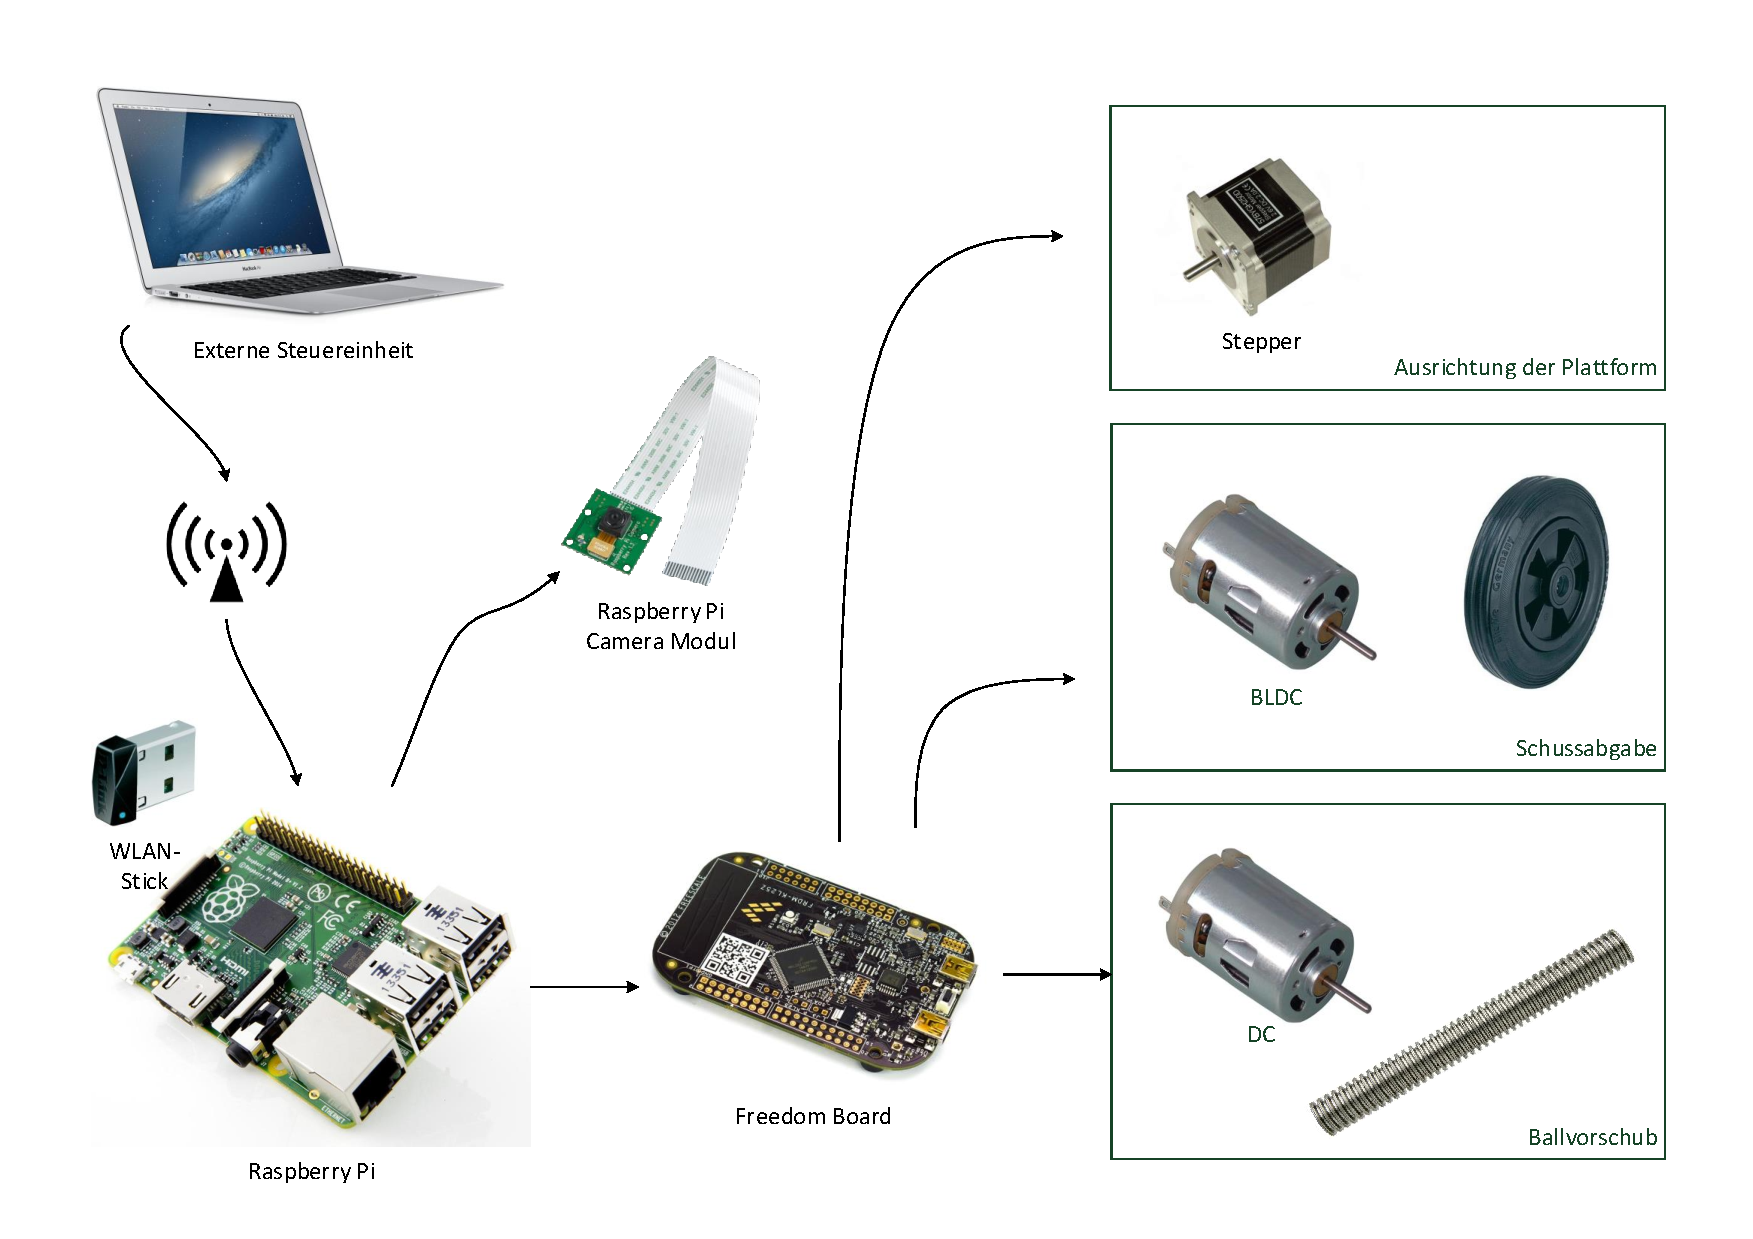
\includegraphics[width=0.9\linewidth]{../../fig/blockdiagramm}
\caption{Blockdiagramm}
\label{fig:blockdiagramm}
\end{figure}
